\hypertarget{_trace_to_mirror_point2_8c}{
\section{/home/mgh/LanlGeoMag/libLanlGeoMag/TraceToMirrorPoint2.c File Reference}
\label{_trace_to_mirror_point2_8c}\index{/home/mgh/LanlGeoMag/libLanlGeoMag/TraceToMirrorPoint2.c@{/home/mgh/LanlGeoMag/libLanlGeoMag/TraceToMirrorPoint2.c}}
}
{\tt \#include $<$stdio.h$>$}\par
{\tt \#include $<$stdlib.h$>$}\par
{\tt \#include \char`\"{}Lgm/Lgm\_\-MagModelInfo.h\char`\"{}}\par
{\tt \#include $<$omp.h$>$}\par


Include dependency graph for TraceToMirrorPoint2.c:\nopagebreak
\begin{figure}[H]
\begin{center}
\leavevmode
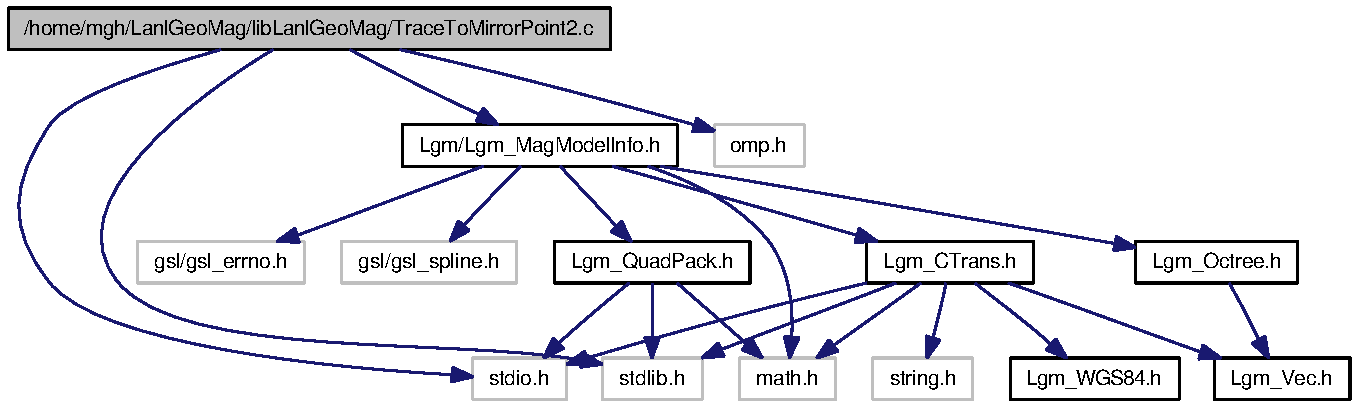
\includegraphics[width=343pt]{_trace_to_mirror_point2_8c__incl}
\end{center}
\end{figure}
\subsection*{Functions}
\begin{CompactItemize}
\item 
int \hyperlink{_trace_to_mirror_point2_8c_f5875fcc683e532736574a4edf7e8545}{Lgm\_\-TraceToMirrorPoint} (\hyperlink{struct_lgm___vector}{Lgm\_\-Vector} $\ast$u, \hyperlink{struct_lgm___vector}{Lgm\_\-Vector} $\ast$v, double $\ast$Sm, double H0, double Bm, double sgn, double tol, \hyperlink{struct_lgm___mag_model_info}{Lgm\_\-MagModelInfo} $\ast$Info)
\end{CompactItemize}


\subsection{Function Documentation}
\hypertarget{_trace_to_mirror_point2_8c_f5875fcc683e532736574a4edf7e8545}{
\index{TraceToMirrorPoint2.c@{TraceToMirrorPoint2.c}!Lgm\_\-TraceToMirrorPoint@{Lgm\_\-TraceToMirrorPoint}}
\index{Lgm\_\-TraceToMirrorPoint@{Lgm\_\-TraceToMirrorPoint}!TraceToMirrorPoint2.c@{TraceToMirrorPoint2.c}}
\subsubsection[{Lgm\_\-TraceToMirrorPoint}]{\setlength{\rightskip}{0pt plus 5cm}int Lgm\_\-TraceToMirrorPoint ({\bf Lgm\_\-Vector} $\ast$ {\em u}, \/  {\bf Lgm\_\-Vector} $\ast$ {\em v}, \/  double $\ast$ {\em Sm}, \/  double {\em H0}, \/  double {\em Bm}, \/  double {\em sgn}, \/  double {\em tol}, \/  {\bf Lgm\_\-MagModelInfo} $\ast$ {\em Info})}}
\label{_trace_to_mirror_point2_8c_f5875fcc683e532736574a4edf7e8545}




Definition at line 25 of file TraceToMirrorPoint2.c.

Here is the call graph for this function:\nopagebreak
\begin{figure}[H]
\begin{center}
\leavevmode
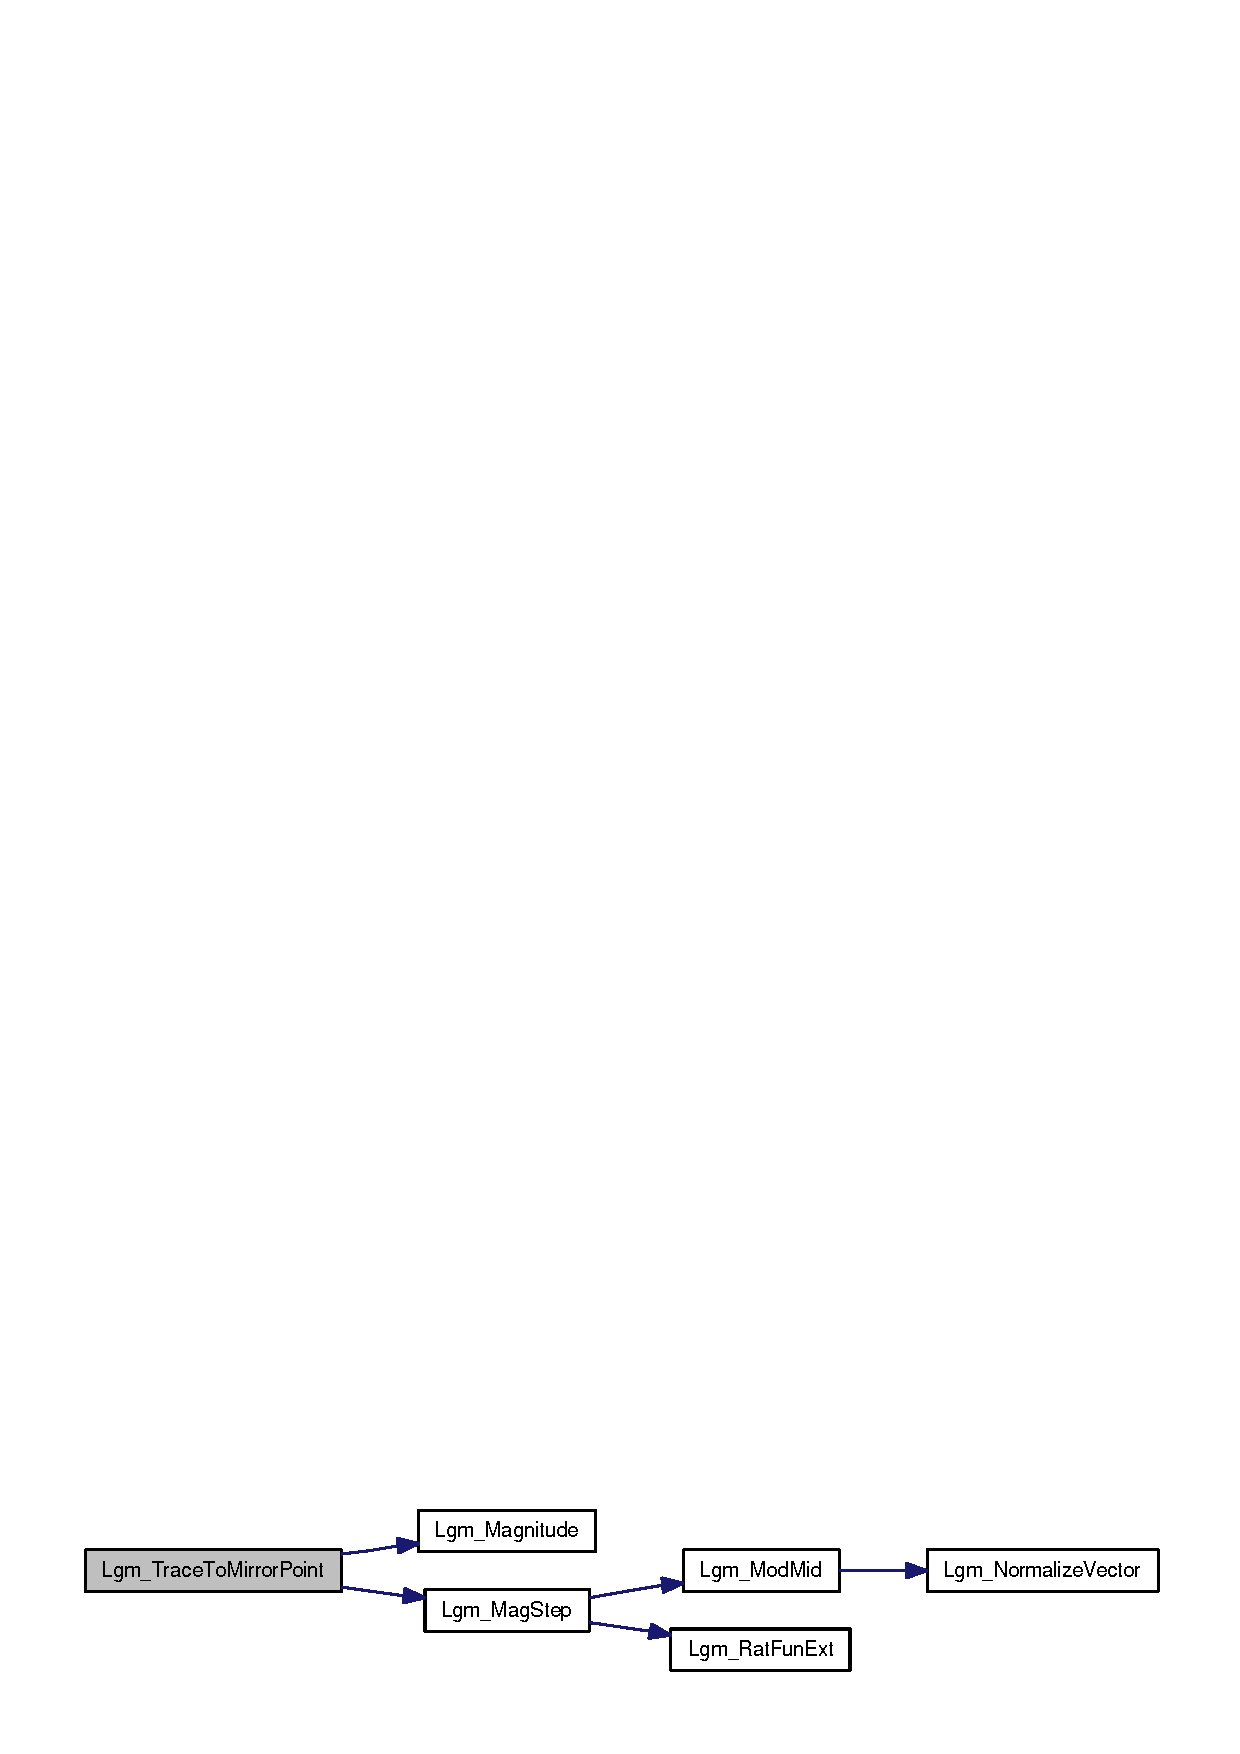
\includegraphics[width=280pt]{_trace_to_mirror_point2_8c_f5875fcc683e532736574a4edf7e8545_cgraph}
\end{center}
\end{figure}


Here is the caller graph for this function:\nopagebreak
\begin{figure}[H]
\begin{center}
\leavevmode
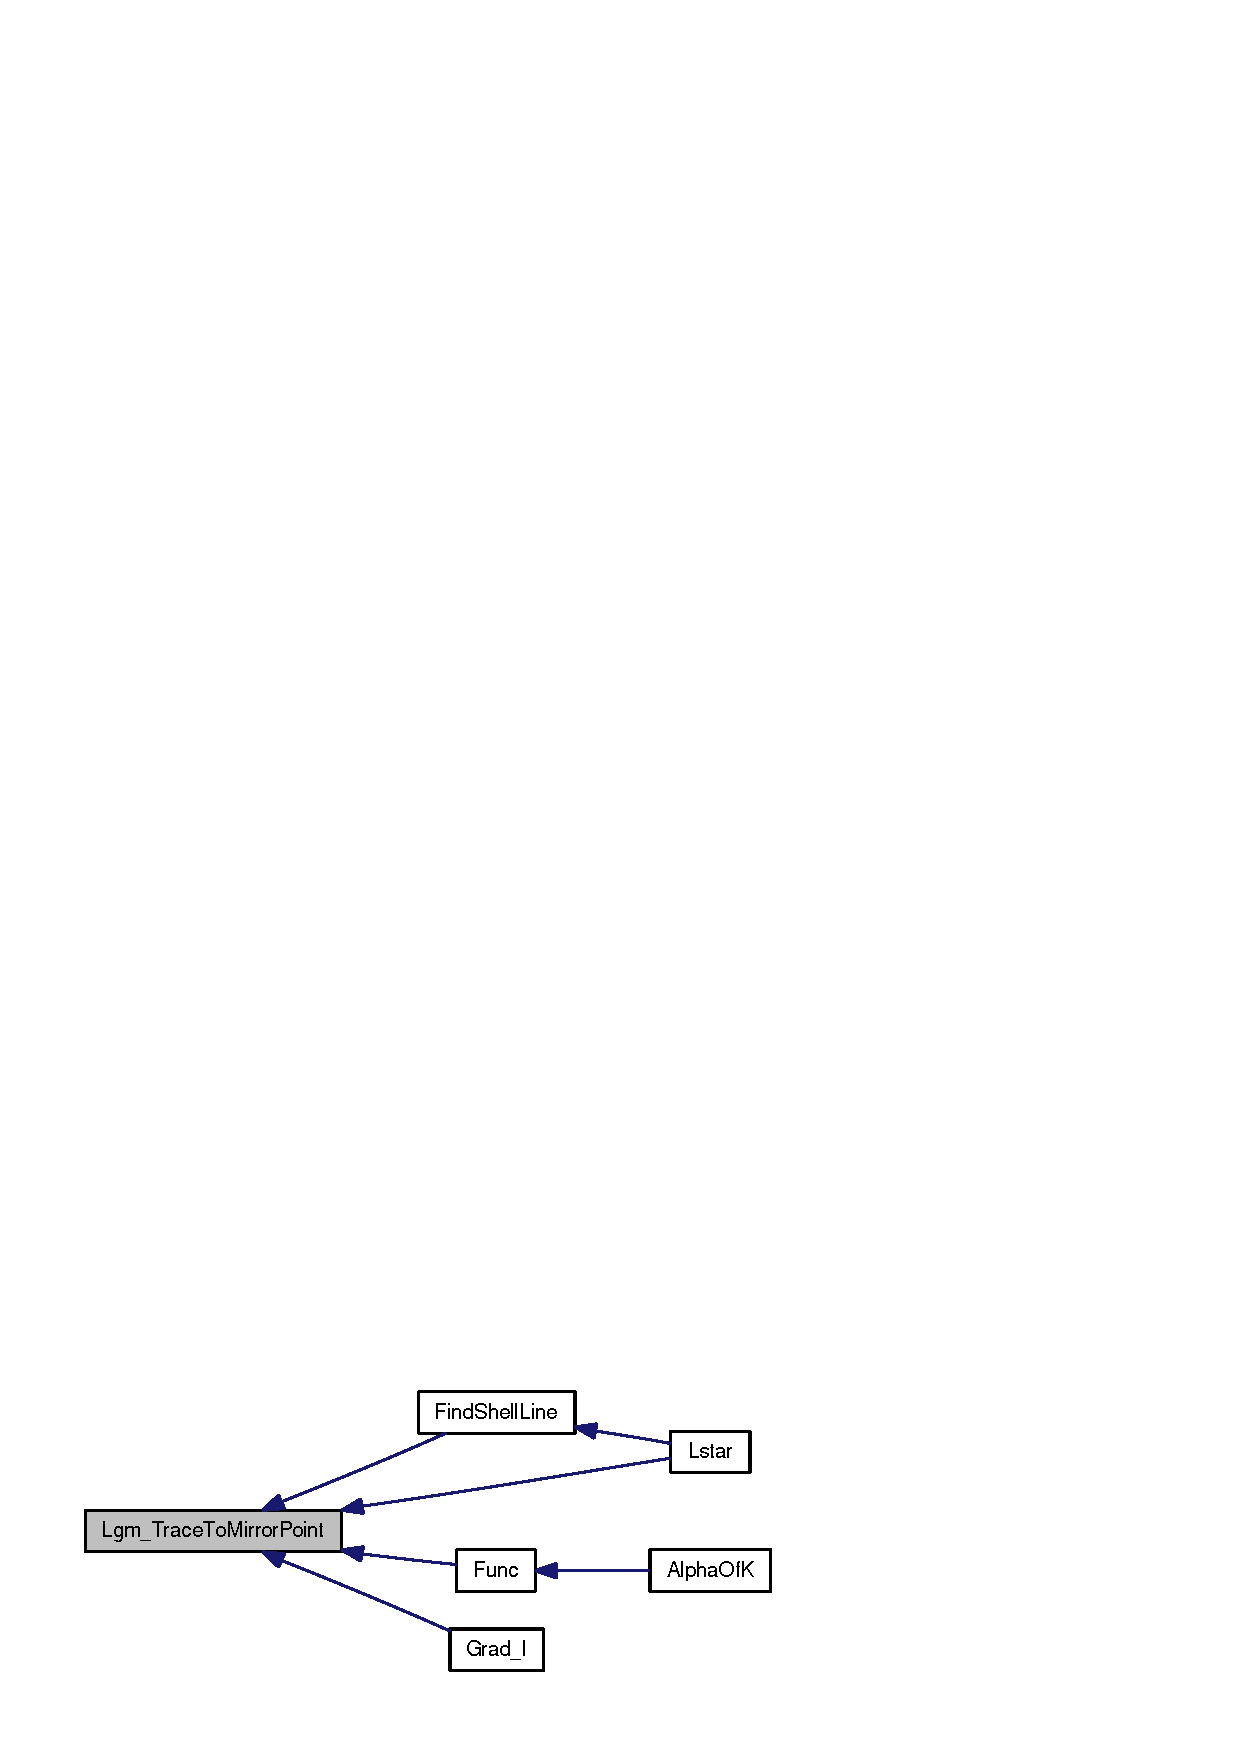
\includegraphics[width=187pt]{_trace_to_mirror_point2_8c_f5875fcc683e532736574a4edf7e8545_icgraph}
\end{center}
\end{figure}
